
\documentclass{beamer}
\usetheme{Montpellier} 
\usecolortheme{dolphin} 
\usepackage{tikz}
\usepackage{tkz-berge}


\title{Our Nice Presentation}
\author{Jordan Blocher, Christopher Linden,  Samantha Hampton}
\date{June 28, 2012}
\institute[2008]{REU - Texas State}

\begin{document}

\frame{\titlepage}
\frame{


\begin{center}
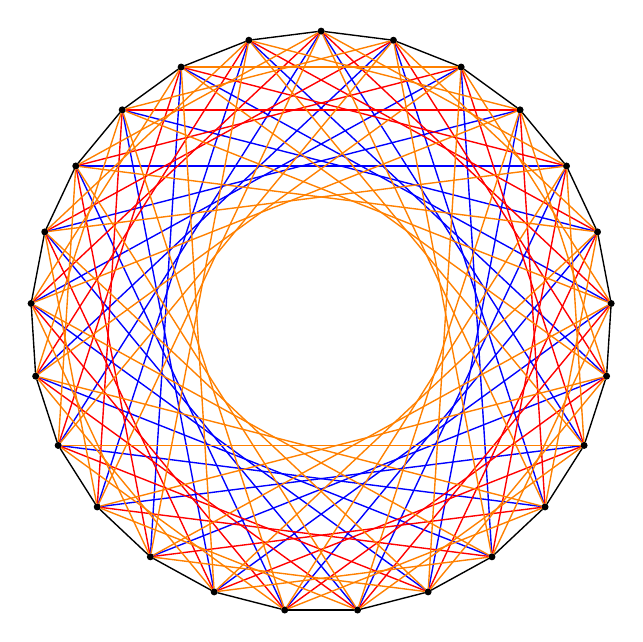
\begin{tikzpicture}[scale=.7]


\GraphInit[vstyle=Simple]
\tikzset{VertexStyle/.append style = {minimum size =2pt, inner sep = 0pt}}


\Vertex[x=187.5pt,y=337.5pt]{0};
\Vertex[x=224.80348307472823pt,y=332.7874741692947pt]{1};
\Vertex[x=259.7630511152573pt,y=318.94600200657953pt]{2};
\Vertex[x=290.1820658893033pt,y=296.8452941132117pt]{3};
\Vertex[x=314.14918882530225pt,y=267.87401924684946pt]{4};
\Vertex[x=330.15847744427305pt,y=233.85254915624213pt]{5};
\Vertex[x=337.2040092642407pt,y=196.91857792939703pt]{6};
\Vertex[x=334.8430876093033pt,y=159.3928028121413pt]{7};
\Vertex[x=323.22405786990294pt,y=123.63310626523908pt]{8};
\Vertex[x=303.0769864163684pt,y=91.88640153769651pt]{9};
\Vertex[x=275.667787843871pt,y=66.14745084375791pt]{10};
\Vertex[x=242.71868290270174pt,y=48.0335271167623pt]{11};
\Vertex[x=206.2999850346457pt,y=38.682794802828326pt]{12};
\Vertex[x=168.70001496535434pt,y=38.682794802828326pt]{13};
\Vertex[x=132.2813170972983pt,y=48.03352711676226pt]{14};
\Vertex[x=99.3322121561291pt,y=66.14745084375782pt]{15};
\Vertex[x=71.92301358363159pt,y=91.88640153769656pt]{16};
\Vertex[x=51.77594213009703pt,y=123.63310626523916pt]{17};
\Vertex[x=40.1569123906967pt,y=159.3928028121413pt]{18};
\Vertex[x=37.795990735759275pt,y=196.91857792939695pt]{19};
\Vertex[x=44.841522555726954pt,y=233.8525491562421pt]{20};
\Vertex[x=60.85081117469775pt,y=267.8740192468495pt]{21};
\Vertex[x=84.81793411069665pt,y=296.8452941132117pt]{22};
\Vertex[x=115.23694888474257pt,y=318.9460020065795pt]{23};
\Vertex[x=150.1965169252717pt,y=332.7874741692946pt]{24};

\SetUpEdge[lw         = .5pt,
            color      = black,
            labelcolor = black]

\Edge(24)(0)
\Edge(0)(1)
\Edge(1)(2)
\Edge(2)(3)
\Edge(3)(4)
\Edge(4)(5)
\Edge(5)(6)
\Edge(6)(7)
\Edge(7)(8)
\Edge(8)(9)
\Edge(9)(10)
\Edge(10)(11)
\Edge(11)(12)
\Edge(12)(13)
\Edge(13)(14)
\Edge(14)(15)
\Edge(15)(16)
\Edge(16)(17)
\Edge(17)(18)
\Edge(18)(19)
\Edge(19)(20)
\Edge(20)(21)
\Edge(21)(22)
\Edge(22)(23)
\Edge(23)(24)

\SetUpEdge[lw         = .5pt,
            color      =blue,
            labelcolor = black]

\Edge(0)(8)
\Edge(2)(10)
\Edge(4)(12)
\Edge(6)(14)
\Edge(8)(16)
\Edge(10)(18)
\Edge(12)(20)
\Edge(14)(22)
\Edge(16)(24)
\Edge(18)(1)
\Edge(20)(3)
\Edge(22)(5)
\Edge(24)(7)
\Edge(1)(9)
\Edge(3)(11)
\Edge(5)(13)
\Edge(7)(15)
\Edge(9)(17)
\Edge(11)(19)
\Edge(13)(21)
\Edge(15)(23)
\Edge(17)(0)
\Edge(19)(2)
\Edge(21)(4)
\Edge(23)(6)

\SetUpEdge[lw         = .5pt,
            color      =red,
            labelcolor = black]

\Edge(0)(6)
\Edge(6)(12)
\Edge(12)(18)
\Edge(18)(24)
\Edge(24)(5)
\Edge(5)(11)
\Edge(11)(17)
\Edge(17)(23)
\Edge(23)(4)
\Edge(4)(10)
\Edge(10)(16)
\Edge(16)(22)
\Edge(22)(3)
\Edge(3)(9)
\Edge(9)(15)
\Edge(15)(21)
\Edge(21)(2)
\Edge(2)(8)
\Edge(8)(14)
\Edge(14)(20)
\Edge(20)(1)
\Edge(1)(7)
\Edge(7)(13)
\Edge(13)(19)
\Edge(19)(0)

\SetUpEdge[lw         = .5pt,
            color      =orange,
            labelcolor = black]

\Edge(0)(4)
\Edge(4)(8)
\Edge(8)(12)
\Edge(12)(16)
\Edge(16)(20)
\Edge(20)(24)
\Edge(24)(3)
\Edge(3)(7)
\Edge(7)(11)
\Edge(11)(15)
\Edge(15)(19)
\Edge(19)(23)
\Edge(23)(2)
\Edge(2)(6)
\Edge(6)(10)
\Edge(10)(14)
\Edge(14)(18)
\Edge(18)(22)
\Edge(22)(1)
\Edge(1)(5)
\Edge(5)(9)
\Edge(9)(13)
\Edge(13)(17)
\Edge(17)(21)
\Edge(21)(0)
\Edge(0)(9)
\Edge(9)(18)
\Edge(18)(2)
\Edge(2)(11)
\Edge(11)(20)
\Edge(20)(4)
\Edge(4)(13)
\Edge(13)(22)
\Edge(22)(6)
\Edge(6)(15)
\Edge(15)(24)
\Edge(24)(8)
\Edge(8)(17)
\Edge(17)(1)
\Edge(1)(10)
\Edge(10)(19)
\Edge(19)(3)
\Edge(3)(12)
\Edge(12)(21)
\Edge(21)(5)
\Edge(5)(14)
\Edge(14)(23)
\Edge(23)(7)
\Edge(7)(16)
\Edge(16)(0)

\end{tikzpicture}
\end{center}

}



\section[Outline]{}
\frame{\tableofcontents}

\section{Introduction}
\subsection{We are going to present our research}

\frame {
	\frametitle{Introduction}
	\begin{itemize}
		\item<1-> The problem at hand 
                     \[
\frac{176}{2197}d^3 + O(d^2) \leq m(d,3) \leq \frac{1}{14-3\sqrt{3}}(d+3)^3 .
\]
		\item<2->Another good argument, after one click
		\item<3->Last one, after another click
	\end{itemize}
}

\section{Next Section}

\subsection{First Sub Section}

\frame {
	\frametitle{Second Frame}
	This text will stay on all pages.
	\only<1>{
		\begin{itemize}
			\item<1->This will only appear on the first page
			\item<1->This is also only for the first page
		\end{itemize}
	}
	\only<2>{
		\begin{itemize}
			\item<2->This will only appear on the second page
		\item<2->This is also only for the second page
		\end{itemize}
      }
}

\subsection{Second Sub Section}

\frame {
	\frametitle{Last Frame}
	This is the last frame
}

\end{document}